\section{ICD Sensing}
\label{sec:sensing}
\begin{figure}[t]
	\centering
	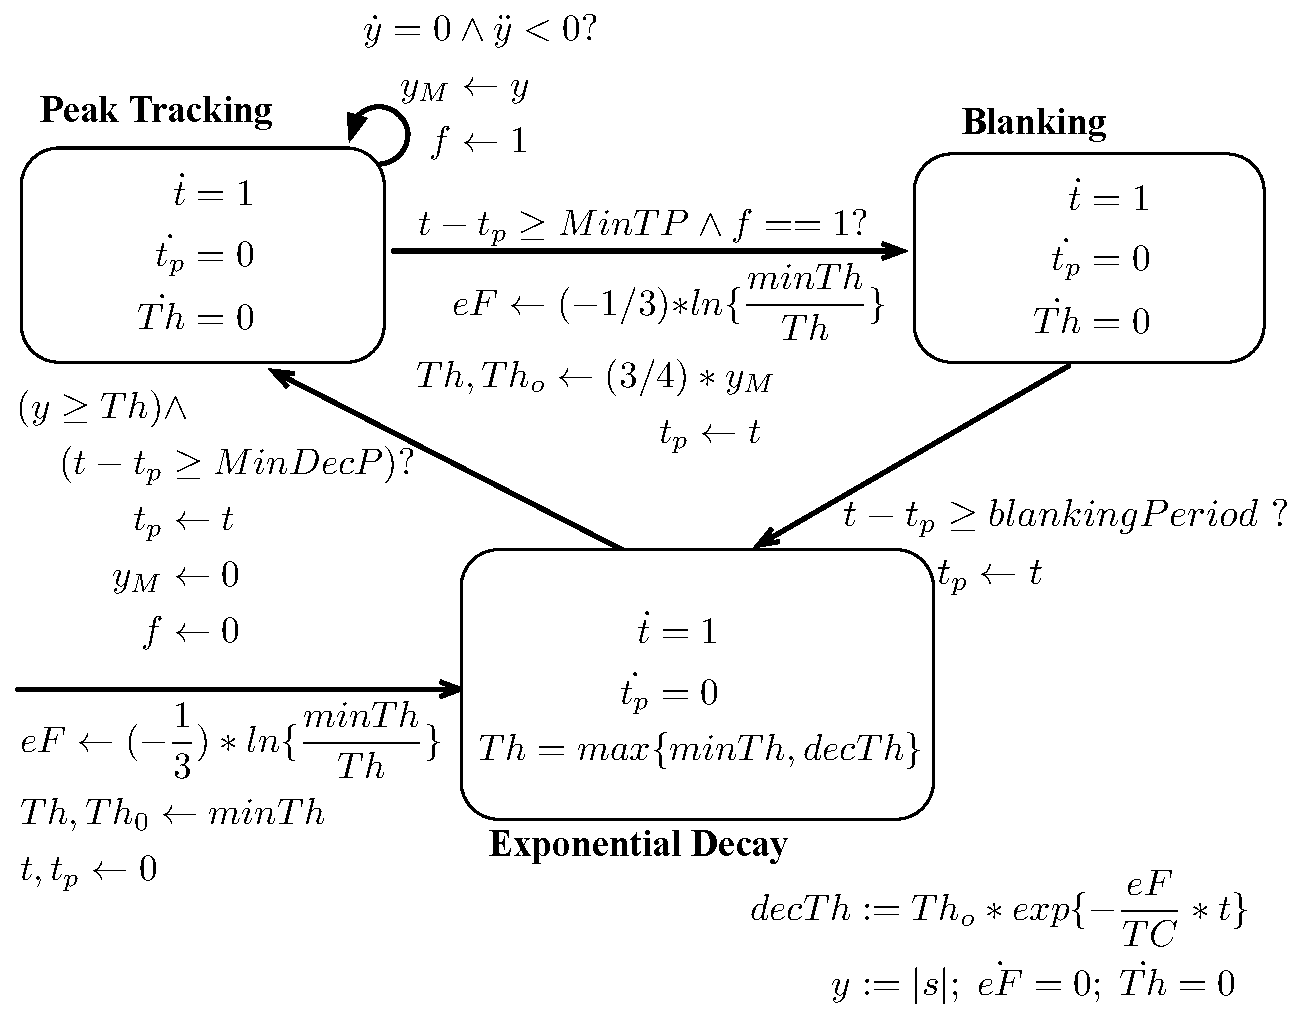
\includegraphics[scale=0.35]{figures/sensingModel}
	\vspace{-10pt}
	\caption{\small $\Sys_{Sense}$. States not shown in a mode have a 0 derivative, e.g., $\dot{eF}=0$ in all modes.}
	\vspace{-10pt}
	\label{fig:sensingModel}
\end{figure}
\begin{figure}[t]
	\centering
	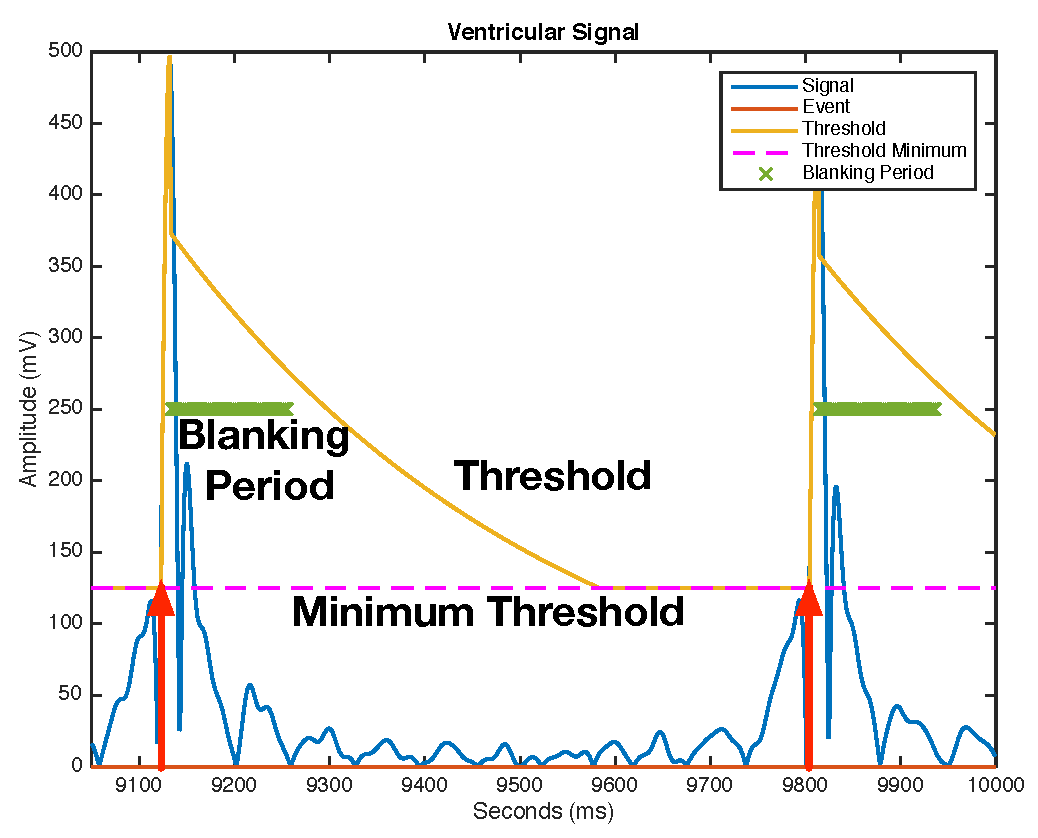
\includegraphics[scale=0.3]{figures/sensingExample}
	\vspace{-10pt}
	\caption{\small Example of dynamic threshold adjustment in ICD sensing algorithm. The shown signal is rectified.}
	\vspace{-10pt}
	\label{fig:sensingExample}
\end{figure}

\emph{Sensing} is the process by which cardiac signals $\egm$ measured through the leads of the \ac{ICD} are converted to cardiac timing events.
The \ac{ICD} sensing algorithm is a threshold-based algorithm which declares events when the signal exceeds a dynamically-adjusted threshold $Th$.
%The threshold is dynamically adjusted in order to operate robustly in complex environments where cardiac events can vary greatly in signal amplitude and frequency, such as during \ac{VF}.

Fig. \ref{fig:sensingModel} shows the model $\Sys_{Sense}$ of the sensing algorithm, and Fig. \ref{fig:sensingExample} illustrates its operation. 
%In Fig. \ref{fig:overview} (ICD Sensing - $\Sys_{Sense}$), states not shown in a mode have a 0 derivative, e.g., $\dot{eF}=0$ in all modes. $y(t) = |\egm(t)|$.
The sensing takes place on the rectified \ac{EGM} signal $y = |\egm|$.
After an event is declared at the current threshold value ($y(t)\geq Th(t)$ in Fig. \ref{fig:sensingModel}), the algorithm tracks the signal in order to measure the next peak's amplitude (mode Peak Tracking).
%During transition, the state to indicate peak discovery is reset ($f=0$). 
For a duration $MinTP$ (min tracking period) the latest peak is saved in $y_M$.
A variable $f$ indicates that a peak was found.
After a peak is found ($f==1$) and after the end of the tracking period, the algorithm enters a fixed \emph{Blanking Period}, during which additional events are ignored.
On that transition, $Th$ and $Th_0$ are set to 3/4 the current value of $y_{M}$ and the exponential factor of decay is updated ($eF=(-1/3)*ln{\frac{minTh}{TH}}$). 
The algorithm then transitions to the Exponential Decay mode in which $Th$ decays exponentially from $Th_0$ to a minimum level:
$Th(t) = \max(minTh, Th_0\cdot exp(-(eF/TC)t)) $.
The algorithm stays in the exponential decay mode for at least a sampling period of $MinDecP$.
Correspondingly, there is a de facto Maximum Decay Period $MaxDecP$ after which the system transitions again to PeakTracking since the signal $y$ is bound to exceed the minimum threshold $minTh$.
Different manufacturers may use a step-wise decay instead of exponential, but the principle is the same.

Local peak detection is modeled via the $\dot{y} = 0 \wedge \ddot{y}<0$ transition.
While $y=|\egm|$ is non-differentiable at 0, the peak will occur away from 0, as shown in Fig. \ref{fig:sensingExample}.
The other states in Fig. \ref{fig:sensingModel} are $t, t_p$ (clocks).
$minTh$ and $TC$ are constant parameters.
\begin{thm}
	\label{thm:sensing}
	$\Sys_{Sense}$ is STORMED.	
\end{thm}
\begin{prf}
	\textbf{(S)} By definition, we only need to consider transitions between different modes to establish separability. 
	For all such transitions, there is a minimum dwell time in the mode before taking the transition, namely $MinTP$ in PeakTracking, $BlankingPeriod$ in Blanking, and  $MinDecP$ in mode ExponentialDecay.
	So the system is separable since there is a uniform minimum flow before jumping.
	\\
	\textbf{(T)} Flows are either constant, (piece-wise) linear, or piece-wise linear and exponential (in the case of $y$ and its derivatives) and therefore are TISG.
	\\
	\textbf{(O)} All the flows, resets and guard sets are definable in $\Lc_{\exp}$.
	(The absolute value and $\max$ functions can be broken down into boolean disjunctions of definable functions, and $t \mapsto \ln(t)$ is o-minimal by o-minimality of $\exp$).
	\\
	\textbf{(RM)} The state is $x = (t, t_p, y, y_M, f, Th, Th_0,eF) \in \Re^8$, and let 
	 $\phi = (\phi_t, \phi_{p}, \phi_y, \phi_m, \phi_f, \phi_{Th},\phi_0,\phi_{eF})$ be the corresponding $\phi$ vector.
	Recall that the \ac{EGM} voltage $\egm$, and so $y=|s|$, is upper-bounded by $V_M$.	
	\\ 
	\textbf{ExponentialDecay $\rightarrow$ PeakTracking}.
	Only $t_p,y_M$ and $f$ are modified, so monotonicity produces the constraint
	 $\phi_p(t-t_p) +\phi_m(0-y_M) + \phi_f(0-1) \stackrel{Want}{\geq} \varepsilon (|t-t_p|+|y_M|+1)$.
	We require the stronger constraint to hold:
	\[\phi_t MinDecP - \phi_m V_M -\phi_f \stackrel{Want}{\geq} \varepsilon(MaxDecP + V_M+1)\]
	\\
	\textbf{PeakTracking $\rightarrow$ PeakTracking}. Only $y_M$ and $f$ are reset. 
	Algebraic manipulation yields $-2V_M\phi_m + \phi_f \stackrel{Want}{\geq} \zeta$
	\\
	\textbf{PeakTracking $\rightarrow$ Blanking}.
	$t_p,eF,Th$ and $Th_0$ are reset, so we get
	\begin{eqnarray*}
	&&\;\phi_p(t-t_p) + \phi_{eF}(-(1/3)\ln(minTh/Th)-eF) 
	\\
	&&+\phi_{Th}(3y_M/4-Th) +\phi_0(3y_M/4-Th_0)
	\\
	&&\geq \varepsilon(|t-t_p|+ |-\frac{1}{3}\ln(\frac{minTh}{Th})-eF|
	\\
	&&+|\frac{3y_M}{4}-Th|+|\frac{3y_M}{4}-Th_0|)
	\end{eqnarray*}
	
	$Th$ is lower-bounded by $minTh$ at all times, and it is naturally upper-bounded by $V_M$ as the threshold should never exceed the largest possible attainable voltage. 
	By the same token, $0\leq eF \leq (1/3)\ln(V_M/minTh)$.
	Then we want the stronger inequality
	\begin{eqnarray*}
	\phi_p MinTP &+& \phi_{eF}(0-(1/3)\ln(V_M/minTh)
	\\
	&+&\phi_{Th}(-V_M) +\phi_0(-V_M)
	\\
	&\geq& \varepsilon(MaxTP+ |\frac{1}{3}\ln(\frac{V_M}{Th})|+|V_M|+|V_M|)
	\end{eqnarray*}
	\\
	\textbf{Blanking $\rightarrow$ ExponentialDecay}. Only $t_p$ is reset and therefore we want, $\phi_p(t-t_p) \geq \varepsilon(|t-t_p|)$, thus the transition yields $\phi_p \geq \varepsilon$.
	
	The above equations can be simultaneously satisfied.
	The simplest thing would be to set all $\phi$ terms that appear above to 0 except for $\phi_t,\phi_p$ which are calculated accordingly.
	
	The flows can be shown to be monotonic along the same $\phi$ and with the same $\varepsilon$.
	For example, in mode ExponentialDecay, only $t,y$ and $Th$ flow.
	Making use of the $V_M$ bound on $y$, we get the constraint
	$\phi_t \tau - 2V_M\phi_y +\phi_{Th}(Th(t+\tau)-Th(t))\geq \varepsilon(\tau+2V_M + |Th(t+\tau)-Th(t)| )$, 
	which yields $\phi_t \geq \varepsilon$, $\phi_y \leq -\varepsilon$ and $\phi_{Th} \geq \varepsilon$. 
	Similarly for the rest.	
\end{prf}

%\begin{thm}
%\label{thm:sensing}
%$\Sys_{Sense}$ is STORMED.	
%\end{thm}
%\begin{prf}
%\textbf{(S)} The guards are separable since each mode has only one guard.
%\\
%\textbf{(T)} The flows are constant, linear or equal to $\pm \egm(t)$ (in the case of $y$) and so are TISG.
%\\
%\textbf{(O)} All the flows, resets and guard sets are definable in $\Lc_{\exp}$.
%(The absolute value and $\max$ functions can be broken down into boolean disjunctions of definable functions).
%In particular, $t \mapsto \ln(t)$ is o-minimal by o-minimality of $\exp$.
%\\
%\textbf{(RM)} The only reset happens on the PeakTracking $\rightarrow$ Blanking transition. 
%The state is $x = (t,Th, eF,Th_0,t_p,y) \in \Re^5$.
%We seek a vector $\phi = (\phi_t, \phi_{Th}, \phi_{eF},\phi_0,\phi_y)$ and $\varepsilon >0$ s.t. 
%\begin{equation}
%\label{eq:sense rm}
%\phi \cdot \left(\begin{matrix}
%t-t \\ (3/4)Th-Th\\ -(1/3)\ln(minTh/Th) - eF\\ (3/4)Th-Th_0\\ t-t_p \\ y-y
%\end{matrix}
%\right) \defeq \phi \cdot \delta \stackrel{Want}{\geq} \varepsilon ||\delta||
%\end{equation} 
%$Th$ is lower-bounded by $minTh$ at all times, and it naturally has an upper bound, since it doesn't make sense to set it above the largest possible voltage. 
%Let that maximum be $maxTh$.
%Then we want the stronger inequality
%\begin{eqnarray*}
%&&\phi_{Th}(-Th/4) + \phi_{eF}(-(1/3)ln(minTh/Th)-eF) 
%\\
%&+& \phi_0(3Th/4-Th_0) + \phi_t (t-t_p) \geq ||\delta||
%\\
%&\geq& -\frac{\phi_{Th}}{4}maxTh + \phi_{eF}(-\frac{2}{3}\ln(minTh/Th)) 
%\\
%&& -\phi_0(2maxTh) + \phi_p(t-t_p)
%\\
%&\stackrel{Want}{\geq}& \varepsilon \left(|\frac{maxTh}{4}| + |\frac{2}{3}\ln(\frac{minTh}{Th})| + |2maxTh| +  \phi_p|t-t_p|\right)
%\end{eqnarray*}
%Since the $\ln$ term is negative and $t\geq t_p$,this yields the constraints:
%$\phi_0,\phi_{Th} < -\varepsilon \text{  and  } \phi_{eF},\phi_t > \varepsilon$.
%%\begin{equation}
%%\label{eq:constraint sense rm}
%%\phi_0,\phi_{Th} < -\varepsilon \text{  and  } \phi_{eF},\phi_t > \varepsilon
%%\end{equation}
%
%The flows are also monotonic along the same $\phi$ and with the same $\varepsilon$.
%For any $t,\tau>0$ and $x\in \stSet$, flow monotonicity is implied by the stronger inequality
%\begin{equation}
%\label{eq:sense fm}
%\phi \cdot \left(\begin{matrix}
%t+\tau-t \\ Th-Th\\ eF - eF\\ Th_0-Th_0\\ t_p-t_p \\ |\egm(t+\tau)|-|\egm(t)|
%\end{matrix}
%\right) \stackrel{Want}{\geq} \varepsilon (\tau + \underbrace{||\egm(t+\tau)|-|\egm(t)||}_{\delta \egm})
%\end{equation} 
%$\implies \phi_t \tau + \phi_y (|\egm(t+\tau)|-|\egm(t)|) \geq \varepsilon (\tau + \left| |\egm(t+\tau)|-|\egm(t)| \right| )$
%Therefore we can choose $\phi_t > \varepsilon$ as before and $\phi_y < -\varepsilon$.
%%We show this for Mode 1 only, the other modes are dealt with similarly.
%%\underline{Mode 1.} For any $t,\tau>0$ and $x\in \stSet$, flow monotonicity 
%%$\phi\cdot(\theta(t+\tau;x)-\theta(t;x)) \geq \varepsilon ||\theta(t+\tau;x)-\theta(t;x)||$ is implied by the stronger inequality
%%\begin{equation}
%%\label{eq:sense fm}
%%\phi \cdot \left(\begin{matrix}
%%t+\tau-t \\ Th-Th\\ eF - eF\\ Th_0-Th_0\\ t_p-t_p \\ -\egm(t+\tau)+\egm(t)
%%\end{matrix}
%%\right) \stackrel{Want}{\geq} \varepsilon (\tau + \underbrace{|\egm(t)-\egm(t+\tau)|}_{\delta \egm})
%%\end{equation} 
%%Observing that the \ac{EGM} signal $\egm$ has naturally defined minimum $\egm_{min}$ and maximum $\egm_{max}$, \eqref{eq:sense fm} is further implied by 
%%\begin{equation}
%%\phi_t\tau + \phi_y(\delta \egm) \geq \phi_t \tau - \phi_y(s_{min} -  s_{max}) \stackrel{Want}{\geq} \varepsilon (\tau +|s_{min} -  s_{max}|)
%%\end{equation}
%%which yields the constraints $\phi_t > \varepsilon, \phi_y < -\varepsilon$, which are consistent with \eqref{eq:constraint sense rm}.
%%The flow monotonicity constraints from the other modes are similarly consistent with \eqref{eq:constraint sense rm}. 
%\end{prf}
